\chapter{Úvod}


Jeden z najzákladnejších problémov, ktoré rieši softvérový vývoj je validácia požiadavkov systému. Tieto požiadavky sú zvyčajne definované pomocou diagramu užitia z UML. 
Bežný postup je navrhnúť model systému podľa týchto požiadaviek za pomoci ostatných diagramov z UML a otestovať ho manuálne implementovaným prototypom. To predstavuje dosť práce jednak s diagramami UML a navyše implementovaný prototyp pravdepodobne stratí veškeré využitie po validácii modelu. Predstavme si však, že vytvoríme model za použitia objektovo orientovaných petriho sietí, ktorý prichádza s možnosťou simulácie modelu. Táto simulácia poskytuje priestor na automatické vytvorenie UML diagramov. Isteže existujú aj rozšírenia UML a metódy na ich prevod do spustiteľnej formy ako MDA methodology, Executable UML (xUML) language alebo Foundational Subset pre xUML, všetky zo zmienených metód však trpia nedostatkom, keď sa spustitelná forma UML modelu v priebehu validácie upravuje, je takmer nemožné vrátiť sa so zmenamy k pôvodnému modelu. 

Hlavným cieľom práce je vytvoriť plnohodnotný nástroj na validáciu modelu, ktorý vygeneruje sekvenčný diagram z jazyka UML. Jazyk UML definuje viac diagramov interakcií z ktorých by sa dalo vybrať, no narozdiel od diagramu interakcií sa dá vygenerovať zo simulácie a navyše je sekvenčný diagram druhý nanajvýš používaný z diagramov UML. Od nástroja sa očakáva, že by mal analyzovať všetky možné scenáre, rozlíšiť redundantné výskyty častí scenárov a agregovať ich, aby obmedzil zobrazované informácie. Ďalej by mal poskytovať intuitívne rozhranie a zachovať všetky informácie zo simulácie ľahko dohľadateľné.

Najzložitejšiu časť generovania sekvenčného diagramu predstavuje nahradzovanie dát potrebných na zostavenie sekvenčného diagramu, ale chýbajúcich v reprezentácii pomocou objektovo orientovaných petriho sietí.

V kapitole.. TODO

\chapter{Objektovo Orientované Petriho Siete}

\section{Trieda a dedičnosť}

\section{Siete}

\subsection{Objektová sieť}

\subsection{Sieť metód}

\subsection{Sieť konstruktoru}

\subsection{Synchrónny port}

\section{Prechod}

\subsection{Podmienky prechodu}

\subsection{Akcia}

\subsection{Stráž}

\section{PNTalk}

TODO

\chapter{Sekvenčné Diagramy}

\chapter{Návrh Implementácie}

V tejto Kapitole budú prednesené hlavné myšlienky ako vytvoriť základné stavebné jednotky sekvenčného diagramu. Popisujúc odkiaľ čerpať potrebné informácie zo simulácie, ako si poradiť z neúplnými informáciami a ako sa vysporiadať z absenciou potrebnej informácie zo simulácie OOPN aby bola škoda na výsledku generátora, čo najnižšia. Kapitola je úzko spätá s predchádzajúcimi dvoma kapitolami, keďže bude ťažiť z možností formalismu OOPN a zároveň z vyjadrovacích schopností jazyka PNTalk na vytvorenie datovej štruktúry pre sekvenčný diagram.

\subsection*{Objekt}
Objekt alebo entita je kľúčová časť v scenáry sekvenčného diagramu. Je to obdĺžnik so štítkom mena vo vnútri v ktorom započne čiara života (lifeline) až do deštrukcie objektu, alebo konca simulácie.

\subsubsection*{Vytvorenie objektu}
Na vytvorenie objektu v sekvenčnom diagrame potrebujeme zo simulácie archivovať minimálne 3 veci:

\begin{enumerate}
	\item čas simulácie v ktorom sa inštancia vytvorí
	\item inštanciu, ktorá inicializovala vytvorenie
	\item triedu vytváranej inštancie
\end{enumerate}
Vďaka týmto údajom sa dá vytvoriť správa v sekvenčnom diagrame, ktorá odsadí objekt vertikálne od počiatku do vzdialenosti podľa času vytvorenia.\\\\
\textit{Poznámka: dodatočne sa bude archivovať aj miesto, kam sa objekt uloží pre počítanie referencií. To sa uplatní pri deštrukcii objektu.}


\subsubsection*{Deštrukcia objektu}
Pre deštrukciu objektu musí zaniknúť posledná referencia na objekt. Kvôli tomu je potreba počítadlo referencií, ktoré však nebude výkonnostne náročné ako plnohodnotný garbage collector. Vďaka selektívnemu výberu prechodov, ktoré manipulujú s miestami, kde sú uložené objekty môžme zredukovať počet opakovaní algoritmu len na vybrané prechody.
\pagebreak

Prechod môže spôsobiť tri veci pri manipulácii s referenciou:
\begin{enumerate}
	\item presunúť referenciu do iného miesta\\
	Pri presune referencie sa len pozmení záznam miesta, v ktorom sa nachádza.
	\item zduplikovať referenciu do iného miesta\\
	Pri zduplikovaní sa vytvorí nový záznam o referencii.
	\item vymazať referenciu \\
	Pri vymazaní sa skontroluje, či nie je počet referencií na objekt nulový. Ak áno, objekt sa deštruuje volaním správy destruct z inštancie s prechodom, ktorý poslednú referenciu vymazal.
\end{enumerate}


\subsubsection*{Konvencia mena}

Objekty v sekvenčných diagramoch sa pomenúvavajú pomocou nasledujúcej konvencie "meno inštancie:meno triedy" vďaka čomu môžu vzniknúť tri typy objektov:


\begin{minipage}[c]{0.45\textwidth}
\begin{enumerate}
	\item Pomenovaný objekt
	\item Anonymný objekt
	\item objekt neznámej triedy
\end{enumerate}
\end{minipage}
\hfill
\begin{minipage}[c]{0.8\textwidth}
	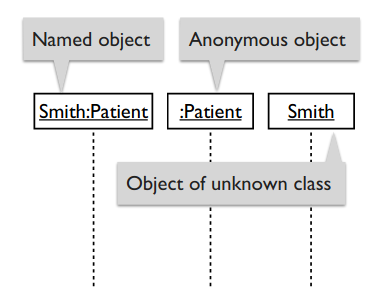
\includegraphics[width=0.45\textwidth]{obrazky-figures/names}
\end{minipage}


syntax jazyka PNTalk vytvára novú inštanciu následovne:

var := classname new.

kde var je dočasná premenná alebo miesto a classname je meno triedy. Problém je zjavný a to, že chýba akákoľvek informácia o mene inštancie. To nám hneď vylúči tretiu možnosť, pretože meno triedy je vždy známe. Varianty sú teda dve a to buď poskladať meno inštancie pomocou známych veličín ako názov miesta, meno triedy, krok simulácie či vygenerovať identifikačné číslo. Druhá varianta je uspokojiť sa s vedomím, že budú vznikať len Anonymné objekty bez názvu inštancie.

\subsection*{Čiara života}
Čiara života alebo inak lifeline je vertikálna čiara reprezentujúca život objektu začína pre každý objekt v dobe vytvorenia a končí deštrukciou objektu, alebo na konci simulácie. Jej vytvorenie je triviálne pokiaľ dokážeme určiť čas vytvorenia a zániku objektu. TODO ref

Je prekrytá bielym obdĺžnikom po dobu, kedy sa metóda objektu nachádza na zásobníku.

\subsubsection*{Na zásobníku}
Doba simulácie po ktorú sa prevádza metóda objektu je viazaná s volaním metód cudzích objektov a preto je nutno archivovať prechody a inštancie, ktoré ich vlastnia. Na tieto prechody potom namapovať prevádzané inštrukcie v chronologickom poradí.

\subsection*{Správa}
Správa vyžaduje poznať odosielateľa, príjemcu a hlavne o aký typ správy sa jedná. Poznáme tri typy:

Synchrónna
Asynchrónna
Odpoveď

zo syntaxe volania metódy pre cudzí objekt evidentne dokážeme zo simulácie odvodiť odosielateľa aj príjemcu.

var methodname: params

kde var je premenná s premennou nesúcou informáciu o mieste s objektom príjemcu. methodname je názov volanej metódy triedy príjemcu. params sú parametre metódy.

odosielateľ je inštancia, ktorá túto akciu zapríčinila svojim prechodom.

Ak metóda vracia hodnotu v simulácii je archivovaná ako odpoveď na správu nesúca údaje o správe na ktorú odpovedá a celú odpoveď.

TODO: Sync vs Async

\subsection*{Cyklus}

K odstráneniu redundantných scenárov značne pomôže zapúzdrenie cyklov, vždy hľadáme v prechodoch najmenší možný ohraničený celok, ktorý sa za sebou sekvenčne niekoľko krát opakuje.

\subsection*{Referovanie a prepájanie diagramov}
Podobne ako pri cykle hľadáme rovnaké, či podobné ohraničené sekvencie prechodov opakujúce sa v simulácii.




\chapter{Implementácia}

\chapter{Záver}


 

